\documentclass[12pt]{article}\usepackage[]{graphicx}\usepackage[dvipsnames]{xcolor}
% maxwidth is the original width if it is less than linewidth
% otherwise use linewidth (to make sure the graphics do not exceed the margin)
\makeatletter
\def\maxwidth{ %
  \ifdim\Gin@nat@width>\linewidth
    \linewidth
  \else
    \Gin@nat@width
  \fi
}
\makeatother

\definecolor{fgcolor}{rgb}{0.345, 0.345, 0.345}
\newcommand{\hlnum}[1]{\textcolor[rgb]{0.686,0.059,0.569}{#1}}%
\newcommand{\hlstr}[1]{\textcolor[rgb]{0.192,0.494,0.8}{#1}}%
\newcommand{\hlcom}[1]{\textcolor[rgb]{0.678,0.584,0.686}{\textit{#1}}}%
\newcommand{\hlopt}[1]{\textcolor[rgb]{0,0,0}{#1}}%
\newcommand{\hlstd}[1]{\textcolor[rgb]{0.345,0.345,0.345}{#1}}%
\newcommand{\hlkwa}[1]{\textcolor[rgb]{0.161,0.373,0.58}{\textbf{#1}}}%
\newcommand{\hlkwb}[1]{\textcolor[rgb]{0.69,0.353,0.396}{#1}}%
\newcommand{\hlkwc}[1]{\textcolor[rgb]{0.333,0.667,0.333}{#1}}%
\newcommand{\hlkwd}[1]{\textcolor[rgb]{0.737,0.353,0.396}{\textbf{#1}}}%
\let\hlipl\hlkwb

\usepackage{framed}
\makeatletter
\newenvironment{kframe}{%
 \def\at@end@of@kframe{}%
 \ifinner\ifhmode%
  \def\at@end@of@kframe{\end{minipage}}%
  \begin{minipage}{\columnwidth}%
 \fi\fi%
 \def\FrameCommand##1{\hskip\@totalleftmargin \hskip-\fboxsep
 \colorbox{shadecolor}{##1}\hskip-\fboxsep
     % There is no \\@totalrightmargin, so:
     \hskip-\linewidth \hskip-\@totalleftmargin \hskip\columnwidth}%
 \MakeFramed {\advance\hsize-\width
   \@totalleftmargin\z@ \linewidth\hsize
   \@setminipage}}%
 {\par\unskip\endMakeFramed%
 \at@end@of@kframe}
\makeatother

\definecolor{shadecolor}{rgb}{.97, .97, .97}
\definecolor{messagecolor}{rgb}{0, 0, 0}
\definecolor{warningcolor}{rgb}{1, 0, 1}
\definecolor{errorcolor}{rgb}{1, 0, 0}
\newenvironment{knitrout}{}{} % an empty environment to be redefined in TeX

\usepackage{alltt}
\usepackage{amsmath,amsfonts,amssymb,graphicx,authblk}
\usepackage[font={footnotesize,singlespacing},labelfont=bf]{caption}
\usepackage{titlesec,blkarray, bm} 
\usepackage{float,afterpage}
\usepackage[running,mathlines]{lineno}
\usepackage[vmargin=1in,hmargin=1in]{geometry}
\usepackage[authoryear,sort]{natbib}
\usepackage[dvipsnames]{xcolor}
\usepackage[nodisplayskipstretch]{setspace} 
\usepackage{hyperref}
\usepackage[section]{placeins}
\usepackage{gensymb}
\usepackage{enumitem}
\usepackage{orcidlink}
\setlist{topsep=.125em,itemsep=-0.15em,leftmargin=0.75cm}
\setlength{\parindent}{0.35in}

\usepackage[sc]{mathpazo} %Like Palatino with extensive math support
\usepackage[subtle]{savetrees}

\usepackage{lineno}
%\renewcommand{\refname}{Literature Cited}
%\renewcommand{\floatpagefraction}{0.9}
%\renewcommand{\topfraction}{0.99}
%\renewcommand{\textfraction}{0.05}

\clubpenalty = 10000
\widowpenalty = 10000

\sloppy 

\usepackage{ifpdf}
\ifpdf
\DeclareGraphicsExtensions{.pdf,.png,.jpg}
\usepackage{epstopdf}
\else
\DeclareGraphicsExtensions{.eps}
\fi

\graphicspath{{/Users/jm200/Library/CloudStorage/Dropbox/Miller Lab/github/ELVI-endophyte-density/Figure/}}
\newcommand{\tom}[2]{{\color{red}{#1}}\footnote{\textit{\color{red}{#2}}}}
\newcommand{\jacob}[2]{{\color{blue}{#1}}\footnote{\textit{\color{blue}{#2}}}}
%\doublespacing



% I cannot get \orcidlink working on my computer so for now replacing this with \textit

%-------------------------------------------------------------------------
\title{Synergistic effect of grass-endophyte symbiosis and herbivory on population demography across a climatic and geographic gradient}
\author[1]{Jacob K. Moutouama\,\textit{0000-0003-1599-1671} \thanks{Corresponding author: jmoutouama@gmail.com}}
\author[1]{Julia Martin}
\author[1]{Ulisses Rizo}
\author[1]{Malcolm Sherwood}
\author[1]{Emily Chong}
\author[1]{Dajanae Pearson}
\author[1]{Alexandra Jimenez Martín}
\author[2]{Josh Fowler}
\author[1]{Ali Campbell}
\author[1]{Chris Oxley}
\author[1]{Karl Schrader}
\author[1]{Tom E.X. Miller\,\textit{0000-0003-3208-6067}}
\affil[1]{Program in Ecology and Evolutionary Biology, Department of BioSciences, Rice University, Houston, TX USA}
\affil[2]{University of Miami, Department of Biology, Miami, FL USA}
\date{} % clear date
%\renewcommand\Authands{ and }

\sloppy

%-------------------------------------------------------------------------
\IfFileExists{upquote.sty}{\usepackage{upquote}}{}
\begin{document}
%\SweaveOpts{concordance=TRUE}
\renewcommand{\baselinestretch}{1.2}
\maketitle
% \bigskip 
%45 character limit on running head
\noindent\textbf{Running header:} Grass-endophyte-herbivory effects across gradients
\bigskip 

\noindent\textbf{Keywords:} demography, range limits

\bigskip 
\noindent\textbf{Submitted to:} \textit{Ecology letters} (Letter)

\bigskip 
\noindent\textbf{Data accessibility statement:} 
If the paper is accepted, all data and computer scripts supporting the results will be archived in a Zenodo package, with the DOI included at the end of the article. 
During peer review, our code (Stan and R) is available at \url{https://github.com/jmoutouama/ELVI-endophyte-density}. 

\bigskip 
\noindent\textbf{Conflict of interest statement:} None.

\bigskip
\noindent\textbf{Authorship statement:}
%J.K.M., A.C. and T.E.X.M. designed the study.
%A.C. and T.E.X.M. collected the data. 
%All authors conducted the statistical analyses and modeling.
%J.K.M. drafted the manuscript, and T.E.X.M contributed to revisions.

\bigskip
\noindent\textbf{Abstract:}\\
\noindent\textbf{Main Text:}\\
\noindent\textbf{Figures: 6}\\
\noindent\textbf{Tables: X}\\
\noindent\textbf{References: X}

\newpage
%\SweaveOpts{concordance=TRUE}
\linenumbers
%-------------------------------------------------------------------------
\spacing{1.25}
\section*{Abstract}
%150 words limit for Ecology letter. The number now is 
Interactions between plants and fungi are ubiquitous in nature and have significant effects on plant fitness.
However, the extent to which variation in fungal frequency affects plant distribution remains understudied. 
Using three cool-season grass species, we combined field experiments on plant populations with variation in leaf endophytic fungi and Bayesian statistics to test whether plant-fungi interactions constrain host demography and, consequently, geographic range limits. 
We found that all vital rates decreased toward the species' range edges, indicating reduced demographic performance in these regions. 
This decline was more pronounced in individuals hosting endophytic symbionts, suggesting that plant-fungi interactions that are beneficial under benign conditions may become parasitic under stressful conditions.
Our results highlight that range expansion may be hindered by the presence of a mutualist.

%--------------------------------------------------------------------
\newpage
\section*{Introduction}
Plant-microbe symbioses are widespread and ecologically important. 
These interactions are famously context-dependent, where the direction and strength of the interaction outcome depends on the environment in which it occurs \citep{fowler2023geographic,hoeksema2015context, bronstein1994conditional}.
Plant-microbe  interactions that are beneficial under stressful conditions  may become parasitic under benign conditions \citep{giauque2019endophyte}.
Under biotic stress (e.g., herbivory), endophyte symbiosis can benefit host plants by facilitating the production of secondary compounds that deter feeding or exert direct toxicity, thereby reducing insect growth, survival, and oviposition \citep{atala2022fungal,bastias2017epichloe,vega2008insect}.
Similarly under abiotic stress (e.g., drought), symbionts can increase their host tolerance  \citep{clay2002evolutionary}.
However, in many plant-microbe interactions, host protection is not guaranteed solely by the presence of a symbionts; rather, the density of the symbiont can determine the effectiveness of this protection \citep{laughton2014combined}. 
Higher endophyte densities may lead to increased resource exploitation by the symbiont, potentially imposing costs on the host, such as reduced growth or reproduction \citep{faeth2009asexual}.
%This cost is often manifested by a reduction in host biomass or reproductive success \citep{faeth2009asexual}, particularly under harsh abiotic conditions \citep{cui2024review}. 
%Ultimately, these context-dependent costs and benefits may underlie the observed distribution of host species.

Context dependence raises the hypothesis that plant-microbe interactions are likely to vary across environmental gradients, from range core to range edge, with significant implications for host range expansion. If microbial symbiosis provides greater benefits under environmental stress, then symbionts could enhance the suitability of range-edge environments, potentially extending host range limits \citep{allsup2023shifting,rudgers2020climate}.
For instance, fungal endophytes improve the survival of \emph{Bromus laevipes}  populations in dry conditions, increasing their drought resistance at the range edge and thereby extending the species' geographic range \citep{david2019soil,afkhami2014mutualist}.
Even if the symbiont does not directly improve host survival, it may still enhance host population growth over time by increasing relative growth and reproduction, potentially offsetting the negative effects of lower survival rates \citep{yule2013costs}.
Conversely, if microbial symbiosis is costly for the host at range edge, symbionts could constrain host range \citep{benning2021microbes,benning2021plant,bennett2022costs}.
%Mutualist limitation reduces population fitness and therefore limits range expansion in \emph{Medicago polymorpha} populations \citep{lopez2021microbial}. 
%Although context dependence, along with spatiotemporal variations in abiotic environmental conditions may reduce the effectiveness of the benefits provided by the symbiont to the host species, our understanding of the mechanisms that alter host-symbiont interactions across species geographic range remains limited.

Ecological studies of plant-microbe symbiosis typically focus on interactions from the plant’s perspective and rarely manipulate symbiont prevalence to assess how symbiont responses to environmental variation may influence host demographic performance across the host's range. 
Symbionts promote their own fitness by affecting host life history traits and enhancing resistance to abiotic and biotic stress \citep{kazenel2015mutualistic, giauque2019endophyte, saikkonen1998fungal}.
Theory predicts that exclusive vertical transmission promotes mutualism and leads to a high prevalence of symbiosis within host populations \citep{fine1975vectors}.
Field-based experiments on plant-fungal symbiosis and population fitness suggest that, within populations, beneficial symbionts may become more prevalent and eventually reach fixation when the recruitment advantages they provide outweigh their reproductive costs under stressful conditions \citep{donald2021context}.
However, populations with lower endophyte prevalence may experience higher rates of symbiont loss among offspring \citep{afkhami2008symbiosis}. 
Therefore, overlooking the role of symbionts and their potential cascading effects on the eco-evolutionary dynamics of host populations could lead to inaccurate predictions of host responses to global change.

Studies on plant–microbe symbiosis often overlook the synergistic effects of abiotic and biotic factors on host dynamics across species' ranges.
Previous research on biotic factors, such as herbivory, has shown that herbivory not only influences the reproductive fitness benefits of symbiosis but also increases symbiont prevalence by enhancing vertical transmission of the fungus to the next generation \citep{gundel2020simulated,agrawal1999transgenerational}.
While informative, these studies have primarily been conducted in greenhouse conditions rather than in field settings or at larger spatial scales, limiting our understanding on how herbivory affect natural populations fitness.
If the ecological context in which herbivory occurs affects population fitness, then the interaction between herbivory and abiotic stressors (e.g., drought) could significantly alter host population dynamics and, consequently, influence species range limitations.

Working across a precipitation gradient in the south-central US, we investigated  how the demographic effects of endophyte symbiosis varied from core to edge of the host range.
To answer these questions, we studied the symbiotic association between  cool-season grass species (\emph{Agrostis hyemalis}, \emph{Elymus virginicus} and \emph{Poa autumnalis}) and their  vertically transmitted fungal symbiont Epichloë sp.. 
Our experiment was design to test the following hypotheses:
\begin{enumerate}
\item We hypothesized that stress associated with aridity and low precipitation would strengthen plant-fungal mutualism, such that the fitness benefits of endophyte symbiosis (survival, growth and fecundity) are maximized at the range edge. 
\item We hypothesized that the stress associated with herbivory would reduce plant-fungal mutualism, such that the fitness costs of endophyte symbiosis (survival, growth and fecundity) are maximized at the range edge. 
\end{enumerate}

%--------------------------------------------------------------------
\section*{Materials and methods}
\subsection*{Study species}
\emph{Agrostis hyemalis}, \emph{Elymus virginicus}, and \emph{Poa autumnalis} (subfamily Pooideae) are cool-season perennial grasses native to woodland and prairie habitats in eastern North America \citep{shaw2011guide}. 
The westernmost range limits of these species correspond to the longitudinal aridity gradient in the central and southern Great Plains (Fig. \ref{fig:site}). 
Throughout their range, these species are symbiotic with seed-transmitted fungal endophytes (\emph{Epichloë} sp. and \emph{E. typhina} subsp. \emph{poae}) \citep{rudgers2009benefits}.
However, \emph{Poa autumnalis} may also acquire endophytes through horizontal transmission \citep{gundel2020simulated}. 
Across natural populations in Texas, endophyte prevalence (the fraction of plants that are endophyte-symbiotic) is 86.55\%, ranging from 77.16\% to 93.5\% in \emph{Agrostis hyemalis} \citep{donald2021context}, 53\% (ranging from 10\% to 100\%) in \emph{Elymus virginicus} \citep{sneck2017variation}, and 96\% in \emph{Poa autumnalis} \citep{rudgers2009fungus}. 
Fungal genotyping indicates that the endophytes are capable of synthesizing secondary compounds such as peramine, loline, and ergot alkaloids, which may confer resistance against drought and herbivory \citep{beaudry1951seed}. 
Additionally, these species are capable of both self-pollination and outcrossing \citep{church1958artificial}. 


\begin{figure}[h!]
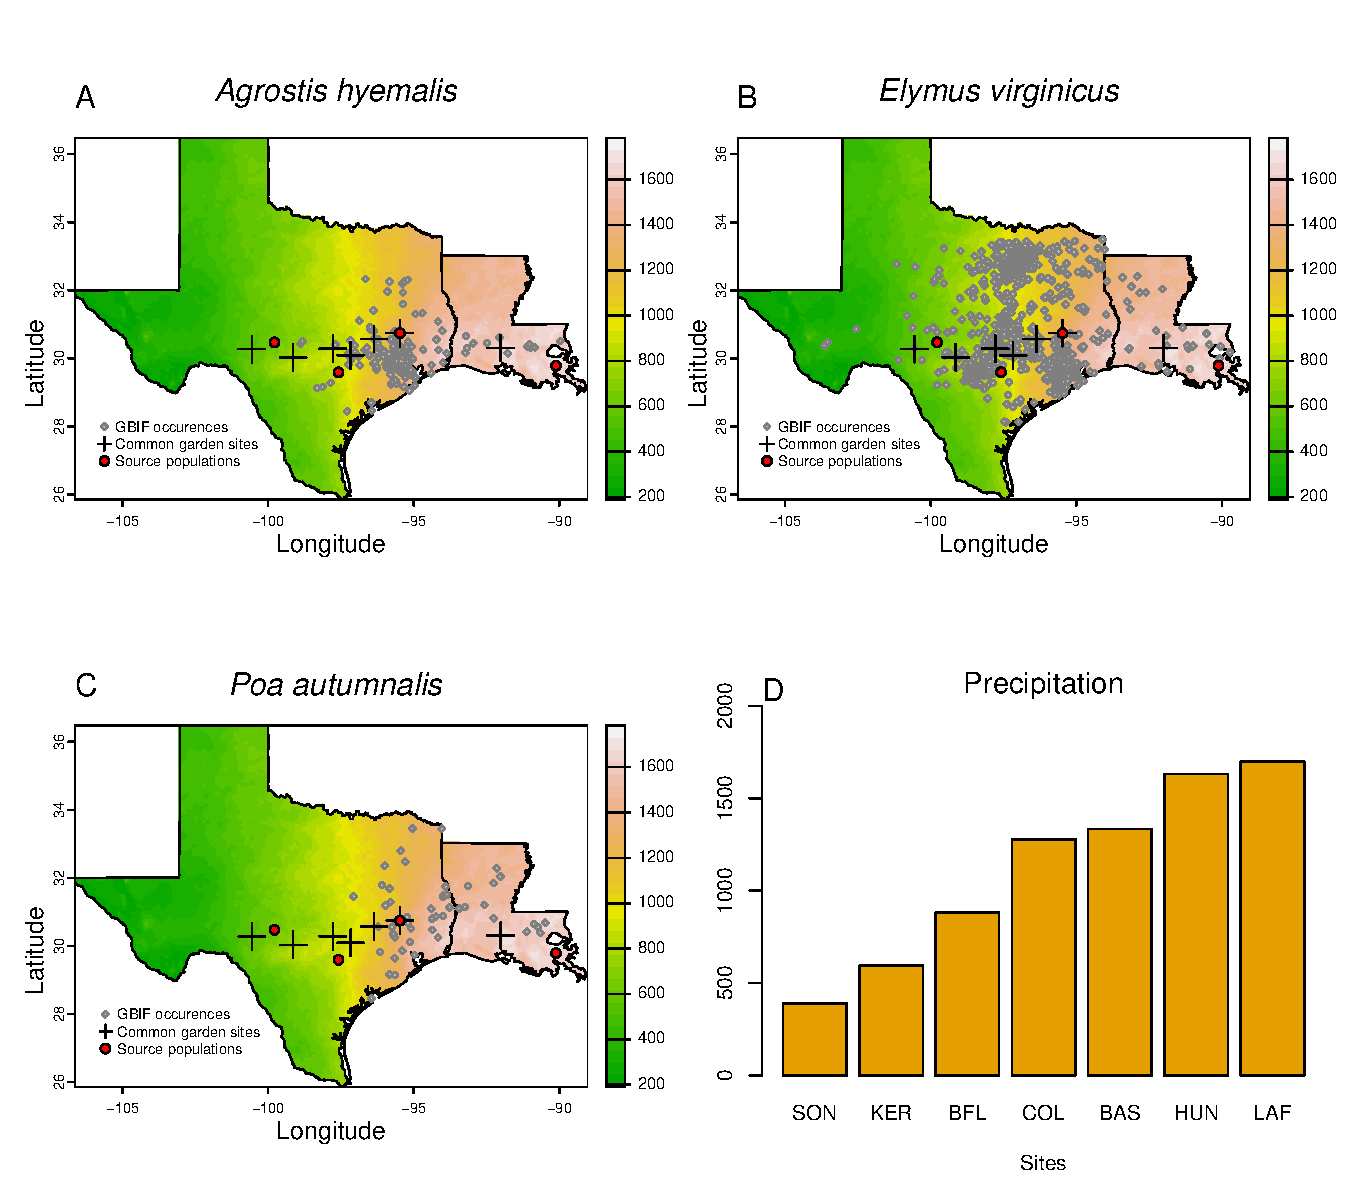
\includegraphics[width=1\textwidth]{clim_map.pdf}
\caption{Distribution of common garden sites across the longitudinal aridity gradient in the central and southern Great Plains for  A) \emph{Agrostis hyemalis}, B) \emph{Elymus virginicus} and C) \emph{Poa autumnalis}.
Red dots represent the locations of source populations, while grey dots represent the GBIF locations of each species across the study area.
D) Cumulative precipitation during the demographic data collection period.}
\label{fig:site}
\end{figure}

\subsection*{Study design}
\paragraph {Experimental Design} 
To understand the demographic effects of endophyte symbiosis from core to edge of the host range, we established  common gardens at 7 sites across the geographic range of \emph {Elymus virginicus} (fig. \ref{fig:site}).
Experimental sites spanned an aridity gradient (temperature gradient).
Common gardens were established in 8 plots per site. 
Plots were 1.5m * 1.5m and the area was tilled of existing vegetation to control for native plant competition.
Plots were also selected in shaded areas under tree canopy or near shrubs to mimic the natural environmental of the species.
In each plot,  we planted 15 individuals  of \emph{E. virginicus} approximately 15 cm deep in an evenly spaced 4*4 grid pattern, with positions randomly assigned. 
For each plot, we randomly assigned a starting endophyte frequency  \jacob{(80\%, 60\%, 40\%, 20\%)}{Do we need a schematic of one replicate
of the experimental design?} and herbivory treatment (herbivores exclusion and herbivores accessibility). 
%Here, the endophyte frequency represents the percentage of  \emph{E. virginicus} individuals that have a symbiont ($E^+$).
We ensured that all plots had comparable quantities of source populations.
After establishing the plots, we watered the plants and recorded initial tiller counts, flowering status and plot position,  endophyte status, source population of each individual plant. 
For herbivory exclusion plots, we enclosed them with 1.2m tall mesh fencing to prevent browsing by vertebrate herbivores and sprayed the plots with insecticide. 
For herbivores accessibility plots (control treatment), we half enclosed the plots with the mesh netting.
We stationed one HOBO MX2307 data logger at each site to collect temperature and volumetric water content in the soil every hour. 

\paragraph {Source populations and Identification of individual endophyte status} 
Plants used  in the common garden experiment were derived from natural populations throughout the native range in the south-central US (fig.\ref{fig:site}, \jacob{Table X}{We need this table  in the Appendix}). 
At each of these natural populations we collected seeds. 
Some of the seeds of \emph{E. virginicus} were heat treated to produce endophyte negative plants ($E^-$) . 
To do so, we placed these seeds  in a drying oven set at 60°C for approximately five days (120 hours). 
While this method eliminates the endophytes from all individuals, it does not affect seed viability. 
All seeds (both heat-treated and non-heat-treated) were planted in the Rice University greenhouse.
Seedlings were regularly fertilized every two weeks. 
The seedlings were then vegetatively propagated to produce enough individuals for your experiment (N = 840).
Before planting in the field, we confirmed the endophyte status ($E^+$ or $E^-$) of all  seedlings using either microscopy or an immunoblot assay. 
This was necessary due to the varying success of the heat treatment and differences in the prevalence of endophytes between the natural populations. 
Leaf tissues were stained with aniline blue lactic acid and viewed under a compound microscope at 200x-400x to identify fungal hyphae. 
The immunoblot assay (Phytoscreen field tiller endophyte detection kit, Agrinostics Ltd. Co.) uses monoclonal antibodies that target proteins of Epichloë spp. and chromagen to visually indicate presence or absence. Both methods yield similar detection rates.  
%The vegetatively cloned plants were distributed across all sites intentionally to allow for comparison of endophyte hyphae densities.

\subsection*{Climatic data}
To characterize the stress gradient with respect to  climatic conditions, we collected the hourly temperature and soil moisture at each site using the HOBO MX2307 data loggers. We used this hourly variable to calculate the daily mean temperature (°C) and soil moisture (\%)(fig. \ref{fig:climate}). 
\jacob{We calculated the mean soil moisture and the coefficient of variation from the time the plants were placed on the ground to the time we collected demographic data}{I will change this  later}. 
The coefficient of variation of soil moisture was estimated to capture season variability in climatic data \citep{medvigy2012trends,meshram2017long}. 

%\begin{figure}[h!]
%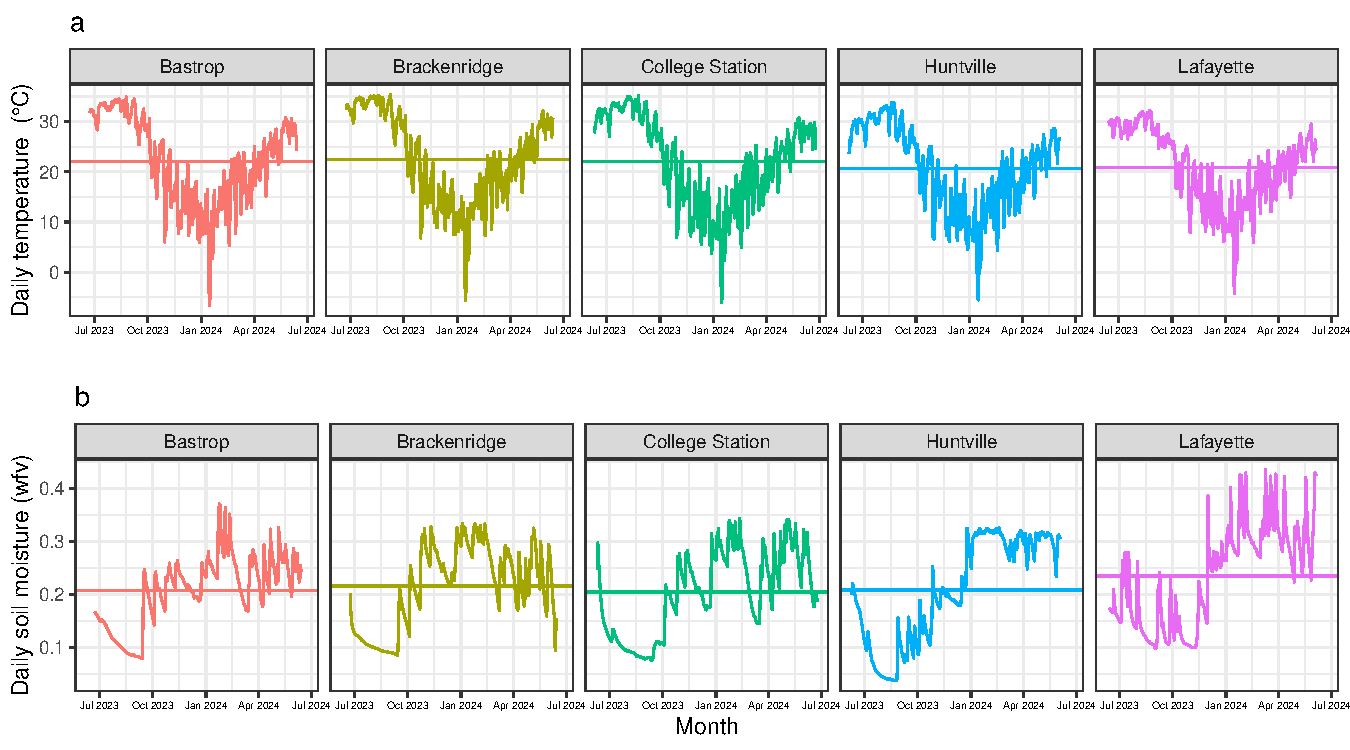
\includegraphics[width=1\textwidth]{climatesite.pdf}
%\caption{Climate variation  across common garden sites. 
%(a) Daily temperature, estimated from average hourly data collected by  HOBO data loggers. 
%(b) Daily  soil moisture, estimated  from average hourly data  collected by  HOBO data loggers. 
%}
%\label{fig:climate}
%\end{figure}

\subsection*{Demographic data}
We collected demographic data including survival, growth, and reproduction during June 2023, which coincided with the flowering season of \emph{E. virginicus}. 
On each individual, survival of plants was recorded as a binary (death or alive) and the size of the plant was recorded as the number of living tillers, indicated by the presence of green coloration. 
We recorded the number of inflorescences per plant and the number of spikelets on up to three inflorescences from three reproducing plants.
We limited the spikelets count to three reproducing tillers per plot due to the time consuming nature of this measurement process. 
We used the number of spikelets for these three tillers to estimate the number the average number of spikelets per plants.

%\subsection*{Endophyte density measurements}
%We collected leaf samples from E+ genotypes that were clonally replicated across two or more sites to quantify endophyte hyphal density and test its associations with host genotype and environmental factors. 
%Relying on clonally replicated genotypes for this analysis allowed us to observe the same genetic individuals in different environments, and partition variation in symbiont density between genetic and environmental sources. 
%
%There were seven unique genotypes of E+ hosts (three PALM, three JLP, one SHS) that were clonally replicated across two or more experimental sites. 
%We collected leaf samples from clonal replicates of these genotypes at up to five sites (excluding COL and SON, where no samples were taken) at the time of the demographic census.
%Samples were taken opportunistically based on survival status and size (we avoided leaf collection from small individuals with few leaves that were vulnerable to mortality).
%We collected 20 leaf samples in total, consisting of one genotype replicated at five sites, three genotypes replicated at three sites, and three genotypes replicated at two sites. 
%
%Samples were placed in a cold cooler in the field and then stored in a -20 freezer until processing.
%In the lab, we examined sections of inner leaf sheath for hyphal density. 
%For each sample, four “peels” of the leaf sheath were placed on a single gridded glass slide (including xmm cells), stained with an aniline blue-lactic acid solution, and viewed under a light microscope at X magnification, following methods in \textcolor{violet}{Sneck et al. 2019}. 
%We randomly sub-sampled cells on the gridded slide, skipping those with less than 25\% leaf peel coverage, until we reached 10 cells for each sample, which amounted to a subsample totaling up to 12mm² per leaf.
%We took digital images of each grid cell. 
%Using ImageJ, we set the scale using the microscope reticle to measure the visible area of the leaf peel within the cell and the total length of the hyphae fragments within the leaf peel.
%This yielded an estimate of endophyte density in the units of length (mm) per area (mm2). 

\subsection*{Models building and models selection}
To assess how stress associated with aridity  affect plant-fungal mutualism, we developed four candidates models for each vital rate (survival, growth, flowering, fertility). 
Each vital rate was modeled with  the  grand mean intercept ($\beta_{0}$), slopes for  variation in each covariate ($\beta_{1}$...$\beta_{3}$) as well as the interaction between covariates ($\beta_{4}$...$\beta_{6}$): 
Each model includes normally distributed random effects for site-to-site  variation ($\phi \sim N(0,\ \sigma_{site})$), plot to plot variation ($\rho \sim N(0,\ \sigma_{site})$), and source-to-source variation that is related to the  provenance of the transplants used to establish the common garden ($\omega \sim N(0,\ \sigma_{source})$) (Eq.\ref{eq:candidates}).
\begin{align}\label{eq:candidates}
\begin{split}
model1 = \beta_{0} + \beta_{1}T_{mean}  + \beta_{2}E + \beta_{3}H + \beta_{4}E*T_{mean} + \beta_{5}H*E +  \beta_{6}H*T_{mean} + \phi + \omega + \rho  \\ 
model2  = \beta_{0} + \beta_{1}T_{CV}  + \beta_{2}E + \beta_{3}H + \beta_{4}E*T_{CV} + \beta_{5}H*E +  \beta_{6}H*T_{CV} +  \phi + \omega + \rho  \\
model3  = \beta_{0} + \beta_{1}M_{mean}  + \beta_{2}E + \beta_{3}H + \beta_{4}E*M_{mean} + \beta_{5}H*E +  \beta_{6}H*M_{mean} + \phi + \omega + \rho \\
model4  = \beta_{0} + \beta_{1}M_{CV}  + \beta_{2}E + \beta_{3}H + \beta_{4}E*M_{CV} + \beta_{5}H*E +  \beta_{6}H*M_{CV} + \phi + \omega + \rho 
\end{split}
\end{align}
 
We modeled survival using a  Bernoulli distribution, growth with a Gaussian distribution, flower with a negative binomial and fertility (number of spikelet) with a negative binomial distribution.
To check whether the fitted models are  compatible with the observed data, we used the posterior predictive checks \citep{gelman2000diagnostic,berkhof2000posterior}. 
All models  do a good job of capturing relevant aspects of the data, such as means, standard deviations, and quantiles (fig.\ref{sup:ppc_surv}, fig.\ref{sup:ppc_growth}, fig.\ref{sup:ppc_spikelet}, fig.\ref{sup:ppc_flowering}).

\jacob{To select the best model for each vital rate, we compared the four models using the leave-one-out cross-validation (LOOCV)} {I need to add something about  difference in  models} \citep{vehtari2017practical}. 
LOOCV combines both validation and training methods. 
In this approach, one observation is used for validation while the training set consists of n-1 observations. 
This process is repeated for each observation, resulting in n estimated models \citep{silva2024robust}. 
The estimate of test error from LOOCV is calculated by averaging the errors across these n models (Eq.\ref{eq:Loo}).
\begin{align}\label{eq:Loo}
\begin{split}
CV_{n}=\frac {1}{n} \sum^{n}_{i=1}{(y_{I}-\hat{y}_{I})^2}
\end{split}
\end{align}

All models were performed in R \citep{RCoreTeam} and Stan \citep{Rstan}.
%%%%%%%%%%%%%%%%%%%%%
% Acknowledgments
%%%%%%%%%%%%%%%%%%%%%
% You may wish to remove the Acknowledgments section while your paper 
% is under review as the Acknowledgments may reveal your identity.
% If you remove this section, you will need to add it back in to your
% final files after acceptance.
\section*{Results}
%\begin{table}[H]
%\caption{Candidate models of  \emph{E. virginicus} vital rates (growth, flowering, spikelet and survival).}
%\label{Table:models}
%\bigskip{}
%\centering
%\begin{tabular}{llll}\hline
%			    Vital rate   &      Model   &     $\Delta$elpd  &  $\Delta$se     \\ \hline
%			 \textbf{Survival} &    \textbf{model3}   &     \textbf{0.0} &     \textbf{ 0.0}    \\
%			Survival &     model2  & -0.5 &   0.5       \\
%			Survival &   model4    & -0.9    &   0.9\\
%			Survival & model1 & -2.2 & 1.9  \\
%		     \textbf{Growth} &   \textbf{model2}&  \textbf{0.0} &  \textbf{0.0} \\
%		    Growth & model4 & 0.0 &  0.8 \\
%		    Growth & model3 & -0.3 &  0.4\\
%		    Growth  &  model1& -0.4 & 0.4\\
%		     \textbf{Flowering} &   \textbf{model2}&  \textbf{0.0}  &  \textbf{0.0}  \\
%		    Flowering & model4 & -4.3 &  1.0\\
%		    Flowering & model3 & -6.5 &  1.4\\
%		     Flowering & model3 & -6.5 &  1.4\\
%		    		     \textbf{Spiket} &   \textbf{model2}&  \textbf{0.0} &  \textbf{0.0}  \\
%		    Spiket & model3 & -0.5 &  0.6\\
%		    Spiket & model1 & -0.7&  1.2\\
%		    Spiket  &  model4 & -1.2 & 1.2\\\hline			    				 			     			     
%\end{tabular}
%\end{table}
%
%\begin{figure}[H]
%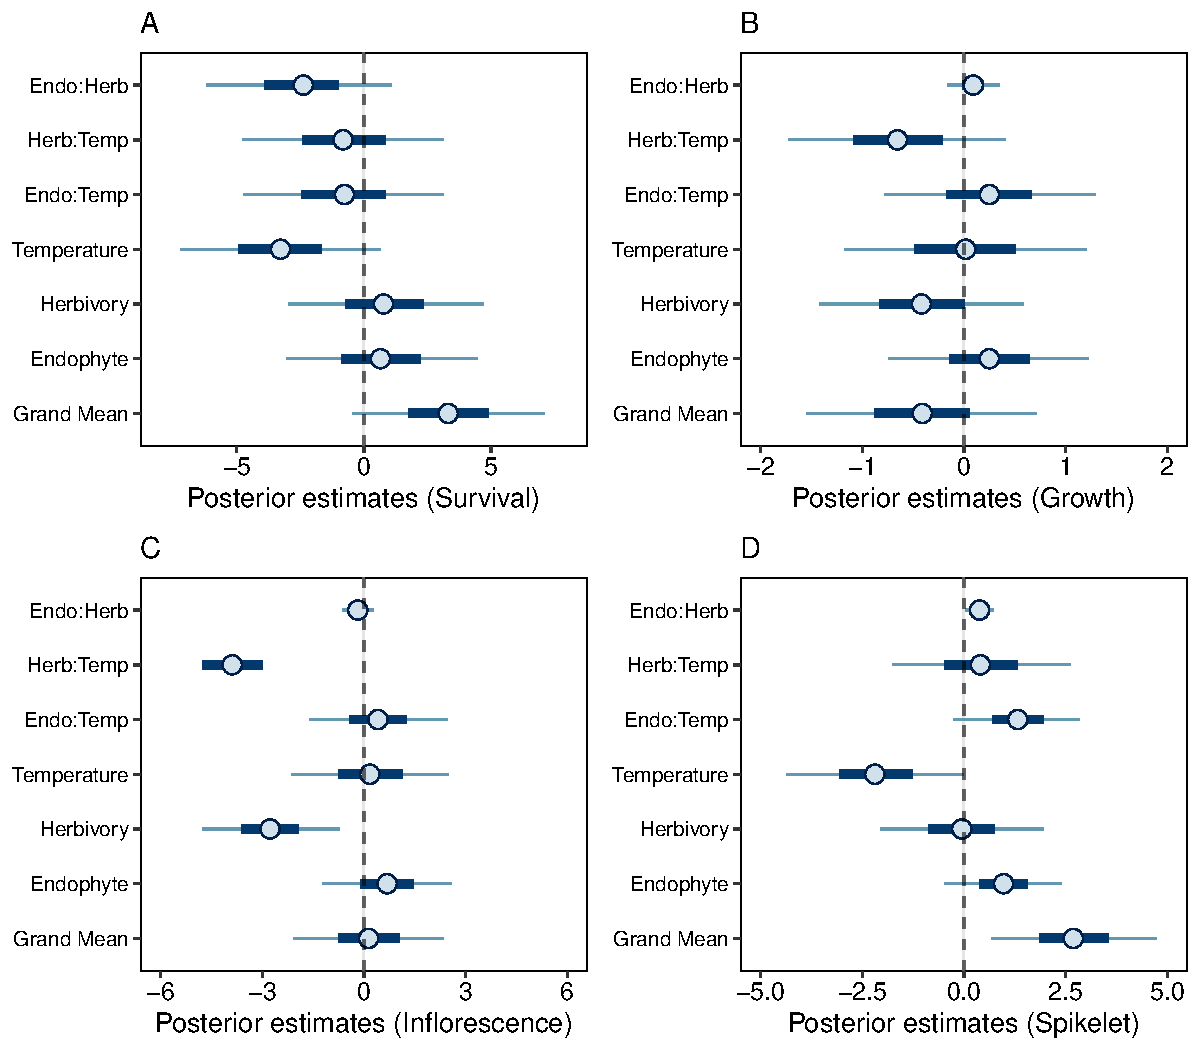
\includegraphics[width=1\textwidth]{Posterior_mean.pdf}
%\caption{Posterior mean estimates for each vital rate. 
%(a) Daily temperature, estimated from average hourly data collected by  HOBO data loggers. 
%(b) Daily  soil moisture, estimated  from average hourly data  collected by  HOBO data loggers. 
%}
%\label{fig:climate}
%\end{figure}
%
%\begin{figure}[H]
%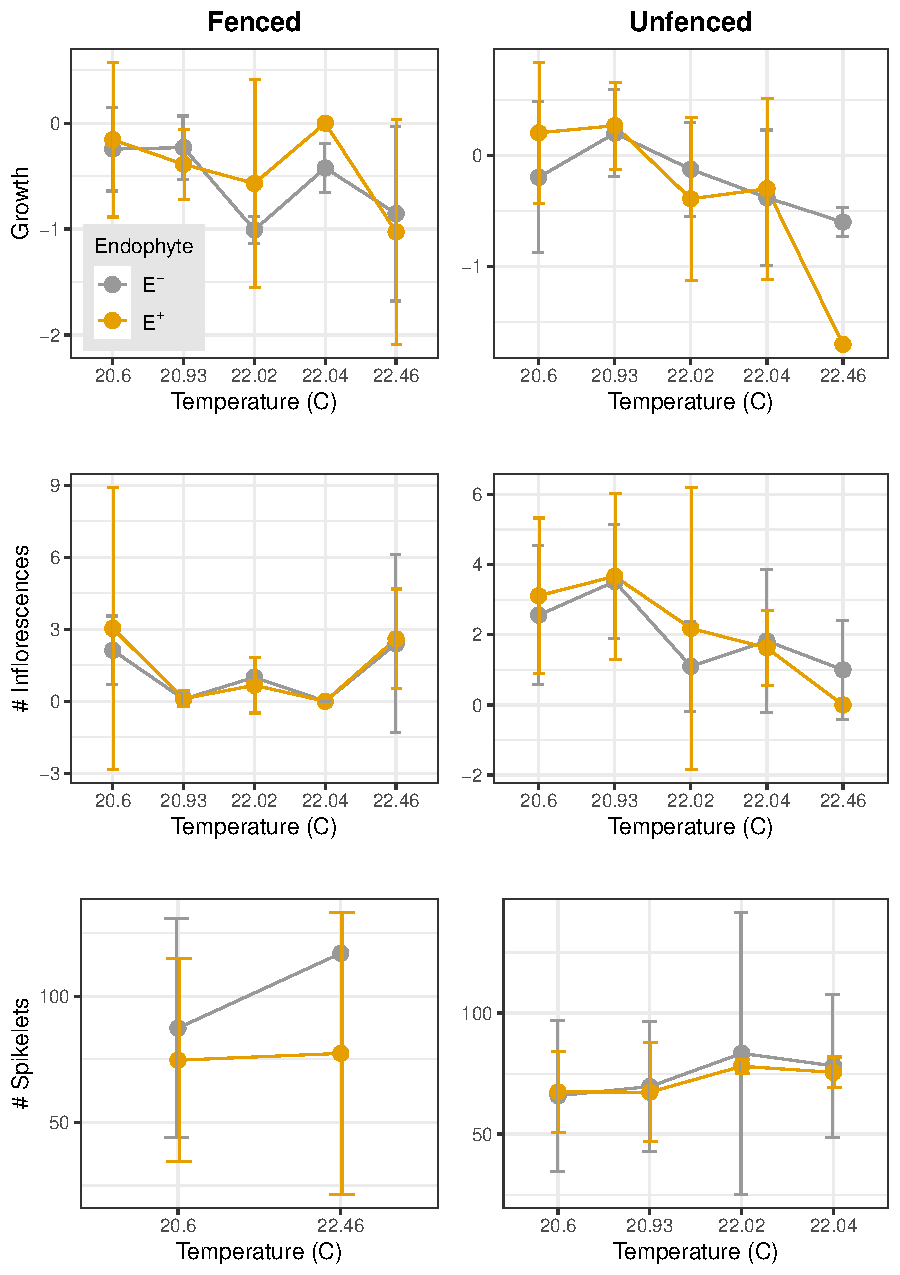
\includegraphics[width=0.9\textwidth]{Fig_temp_mean.pdf}
%\caption{Variation in vital rates across a temperature gradient.
%}
%\label{fig:vital}
%\end{figure}
%
%

\section*{Acknowledgements}
This research was supported by National Science Foundation Division of Environmental Biology awards 1543651 and 1754468 and by the Rice University Faculty Initiatives Fund.



\newpage
\bibliographystyle{apalike}
\bibliography{References}
%--------------------------------------------------------------------
\newpage
\clearpage 
\setcounter{equation}{0}
\setcounter{figure}{0}
\setcounter{section}{0}
\setcounter{table}{0}
\renewcommand{\theequation}{S.\arabic{equation}}
\renewcommand{\thetable}{S-\arabic{table}}
\renewcommand{\thefigure}{S-\arabic{figure}}
\renewcommand{\thesection}{S.\arabic{section}}

\centerline{\Large{\textbf{Supporting Information}}}

%\section {Supporting Figures}
%
%\begin{figure}[H]
%		\centering
%		\includegraphics[width=0.95\linewidth]{Figures/fig_tas_past_present_future.pdf}
%		\caption{Temperature variation across the study sites from 1990 to 2100,
%		ds: Dormant season, dg: Growing season.}
%		\label{Sup:temp_variation}
%\end{figure}
%
%\begin{figure}[H]
%		\centering
%		\includegraphics[width=0.95\linewidth]{Figures/fig_pr_past_present_future.pdf}
%		\caption{Precipitation variation across the study sites from 1990 to 2100.
%		ds: Dormant season, dg: Growing season.}
%		\label{Sup:pr_variation}
%\end{figure}
%
%\begin{figure}[H]
%		\centering
%		\includegraphics[width=0.95\linewidth]{Figures/MIROC.pdf}
%		\caption{Past, Observed, present and future (MIROC Model) climate data across the study area.}
%		\label{Sup:projectionMIROC}
%\end{figure}
%
%\begin{figure}[H]
%		\centering
%		\includegraphics[width=0.99\linewidth]{Figures/ACCESS.pdf}
%		\caption{Past, Observed, present and future (ACCESS Model) climate data across the study area.}
%		\label{Sup:projectionACCESS}
%\end{figure}
%
%\begin{figure}[H]
%		\centering
%		\includegraphics[width=0.99\linewidth]{Figures/CESM1.pdf}
%		\caption{Past, Observed, present and future (CESM1 Model) climate data across the study area.}
%		\label{Sup:projectionCESM1}
%\end{figure}
%
%\begin{figure}[H]
%		\centering
%		\includegraphics[width=0.99\linewidth]{Figures/CMCC.pdf}
%		\caption{Past, Observed, present and future (CMCC Model) climate data across the study area.}
%		\label{Sup:projectionCMCC}
%\end{figure}
%
%\begin{figure}[H]
%		\centering
%		\includegraphics[width=0.959\linewidth]{Figures/site_year_weather.pdf}
%		\caption{Climate variation across the study sites during the monitoring period.}
%		\label{Sup:climate_variation}
%\end{figure}


\end{document}
